\documentclass{article}



\usepackage{fullpage}
\usepackage{nopageno}
\usepackage{amsmath}
\usepackage{amsfonts}
\usepackage{graphicx}
\usepackage{framed}
\usepackage{xcolor}

\definecolor{dark_red}{rgb}{0.5,0.0,0.0}
\definecolor{dark_green}{rgb}{0.0,0.5,0.0}
\definecolor{dark_blue}{rgb}{0.0,0.0,0.5}

\newcommand{\dr}[1]{\textcolor{dark_red}{#1}}
\newcommand{\dg}[1]{\textcolor{dark_green}{#1}}
\newcommand{\db}[1]{\textcolor{dark_blue}{#1}}


\begin{document}

%\section*{Some Review and missed topics}

%\subsection*{Periodic Functions}
%
%Given a periodic function \(f(x)\) with a period of \(T\), then for all \(x \in \mathbb{R}\), 
%\[\cdots = f(x - 3T) = f(x - 2T) = f(x - T) = f(x) = f(x + T) = f(x + 2T) = f(x + 3T) = \cdots\]
%
%\begin{itemize}
%\item If \(m\) and \(c\) are arbitrary real numbers, and \(m \neq 0\), then the period of the function \(g(x) = f(mx + c)\) is \(\frac{T}{|m|}\). 
%\item For the periodic function \(f(x)\), \(x\) has to increase or decrease by the amount \(T\) for \(f(x)\) to repeat itself. 
%\item In the case of \(g(x) = f(mx + c)\), the expression \(mx + c\) has to increase or decrease by the amount \(T\) for \(g(x)\) to repeat itself. 
%	\begin{itemize}
%	\item[*] For \(mx + c\) to increase or decrease by the amount \(T\), \(mx\) has to increase or decrease by the amount \(T\) as \(c\) does not change. 
%	\item[*] For \(mx\) to increase or decrease by the amount \(T\), \(x\) has to increase or decrease by the amount \(\left|\frac{T}{m}\right| = \frac{T}{|m|}\). 
%	\item[*] The increase of \(\frac{T}{|m|}\) is the period of \(g(x)\).
%	\end{itemize}
%\end{itemize}
%
%\textbf{Examples:}
%\begin{itemize}
%\item Let \(g(x) = \sin(57^\circ - 4x)\). Firstly, \(f(x) = \sin(x)\) has a period of \(360^\circ\). For \(g(x)\) to repeat itself, \(57^\circ - 4x\) must change by \(360^\circ\), so \(x\) must change by \(\frac{360^\circ}{|-4|} = 90^\circ\). The period of \(g(x)\) is \(90^\circ\).
%\end{itemize}



\section*{Vectors Concluded}

\subsection*{Displacement between two points}

\begin{tabular}{cc}
\parbox{0.5\textwidth}{
Given two points \(A(x_1,y_1)\) and \(B(x_2,y_2)\), the displacement \(\mathbf{d}\) from point \(A\) to point \(B\) is \(\mathbf{d} = \langle x_2 - x_1, y_2 - y_1 \rangle\). The horizontal component of \(\mathbf{d}\) is the change in the \(x\)-coordinate from \(A\) to \(B\), while the vertical component of \(\mathbf{d}\) is the change in the \(y\)-coordinate from \(A\) to \(B\). \\
\textbf{Examples:}
\begin{itemize}
\item The displacement from \(A(-3,2)\) to \(B(4,-1)\) is \(\mathbf{d} = \langle 7, -3 \rangle\).
\item The displacement from \(A(11,-2)\) to \(B(3,5)\) is \(\mathbf{d} = \langle -8, 7 \rangle\).
\item The displacement from \(A(5,8)\) to \(B(7,0)\) is \(\mathbf{d} = \langle 2, -8 \rangle\).
\end{itemize}
} & \parbox{0.5\textwidth}{
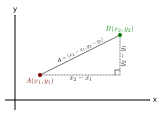
\includegraphics[width = 0.5\textwidth]{displacement_between_points}
}
\end{tabular}

Also, given a point \(A(x,y)\) and a displacement vector \(\mathbf{d} = \langle d_x, d_y \rangle\), the resultant point \(B\) from moving through a displacement of \(\mathbf{d}\) starting from point \(A\) is \(B(x + d_x, y + d_y)\). \\
\textbf{Examples:}
\begin{itemize}
\item Starting from point \(A(6,-2)\), moving a displacement of \(\mathbf{d} = \langle -3, 5 \rangle\) arrives at the point \(B(3,3)\).
\item Starting from point \(A(-1,-7)\), moving a displacement of \(\mathbf{d} = \langle 2, 4 \rangle\) arrives at the point \(B(1,-3)\).
\item Starting from point \(A(-4, 7)\), moving a displacement of \(\mathbf{d} = \langle 4, -1 \rangle\) arrives at the point \(B(0,6)\).
\end{itemize}



%\subsection*{Component vector math}
%
%\textbf{Examples:}
%\begin{itemize}
%\item \(\langle 5, -8 \rangle + \langle -2, 6 \rangle = \langle (5) + (-2) , (-8) + (6) \rangle = \langle 3 , -2 \rangle\)
%\item \(3 \langle -2, 4 \rangle = \langle (3)(-2), (3)(4) \rangle = \langle -6, 12 \rangle\)
%\item \(-7 \langle 5, 2 \rangle + 5 \langle 2, 3 \rangle = \langle -35, -14 \rangle + \langle 10, 15 \rangle = \langle -25, 1 \rangle\)
%\item \(\|\langle 6, 8 \rangle\| = \sqrt{6^2 + 8^2} = \sqrt{36 + 64} = \sqrt{100} = 10\)
%\end{itemize}



%\subsection*{Length and Direction}
%
%Given a vector \(\mathbf{v}\) with:
%\begin{itemize}
%\item A length of \(r\), and an angle of \(\theta\) above the positive x-axis: \(\mathbf{v} = \langle r\cos\theta, r\sin\theta \rangle\)
%\item A length of \(r\), and an angle of \(\theta\) right of the positive y-axis: \(\mathbf{v} = \langle r\sin\theta, r\cos\theta \rangle\)
%\item A length of \(r\), and an angle of \(\theta\) left of the positive y-axis: \(\mathbf{v} = \langle -r\sin\theta, r\cos\theta \rangle\)
%\item A length of \(r\), and an angle of \(\theta\) above the negative x-axis: \(\mathbf{v} = \langle -r\cos\theta, r\sin\theta \rangle\)
%\item A length of \(r\), and an angle of \(\theta\) below the negative x-axis: \(\mathbf{v} = \langle -r\cos\theta, -r\sin\theta \rangle\)
%\item A length of \(r\), and an angle of \(\theta\) left of the negative y-axis: \(\mathbf{v} = \langle -r\sin\theta, -r\cos\theta \rangle\)
%\item A length of \(r\), and an angle of \(\theta\) right of the negative y-axis: \(\mathbf{v} = \langle r\sin\theta, -r\cos\theta \rangle\)
%\item A length of \(r\), and an angle of \(\theta\) below the positive x-axis: \(\mathbf{v} = \langle r\cos\theta, -r\sin\theta \rangle\)
%\end{itemize}
%
%Given a vector \(\mathbf{v} = \langle x, y \rangle\), the length is \(\|\langle x, y \rangle\| = \sqrt{x^2 + y^2}\)
%\begin{itemize}
%\item When \(x \geq 0\) and \(y \geq 0\), the angle above the positive x-axis is \(\tan^{-1}(|y|/|x|)\), and the angle to the right of the positive y-axis is \(\tan^{-1}(|x|/|y|)\).
%\item When \(x \leq 0\) and \(y \geq 0\), the angle to the left of the positive y-axis is \(\tan^{-1}(|x|/|y|)\), and the angle above the negative x-axis is \(\tan^{-1}(|y|/|x|)\).
%\item When \(x \leq 0\) and \(y \leq 0\), the angle below the negative x-axis is \(\tan^{-1}(|y|/|x|)\), and the angle to the left of the negative y-axis is \(\tan^{-1}(|x|/|y|)\).
%\item When \(x \geq 0\) and \(y \leq 0\), the angle to the right of the negative y-axis is \(\tan^{-1}(|x|/|y|)\), and the angle below the positive x-axis is \(\tan^{-1}(|y|/|x|)\).
%\end{itemize}
%
%
%\textbf{Examples:}
%\begin{itemize}
%\item Given a vector \(\mathbf{v}\) where \(\|\mathbf{v}\| = 5\) and the direction is \(\theta = 30^\circ\) above the positive x-axis, then \(\mathbf{v} = \langle 5\cos 30^\circ, 5\sin 30^\circ \rangle \approx \langle 4.330, 2.500 \rangle\)
%\item Given a vector \(\mathbf{v}\) where \(\|\mathbf{v}\| = 6\) and the direction is \(\theta = 20^\circ\) left of the negative y-axis, then \(\mathbf{v} = \langle -6\sin 20^\circ, -6\cos 20^\circ \rangle \approx \langle -2.052, -5.638 \rangle\)
%\item Given a vector \(\mathbf{v}\) where \(\|\mathbf{v}\| = 7\) and the direction is \(\theta = 25^\circ\) beneath the positive x-axis, then \(\mathbf{v} = \langle 7\cos 25^\circ, -7\sin 25^\circ \rangle \approx \langle 6.344, -2.958 \rangle\)
%\end{itemize}
%
%\begin{itemize}
%\item Given the vector \(\mathbf{v} = \langle -2, 8 \rangle\), then the length is \(\|\mathbf{v}\| = \sqrt{(-2)^2 + 8^2} = \sqrt{4 + 64} = \sqrt{68} \approx 8.246\), and the direction can be quantified as either \(\theta = \tan^{-1}(2/8) \approx 14.04^\circ\) left of the positive y-axis, or \(\theta = \tan^{-1}(8/2) \approx 75.96^\circ\) above the negative x-axis.
%\item Given the vector \(\mathbf{v} = \langle -3, -5 \rangle\), then the length is \(\|\mathbf{v}\| = \sqrt{(-3)^2 + (-5)^2} = \sqrt{9 + 25} = \sqrt{34} \approx 5.831\), and the direction can be quantified as either \(\theta = \tan^{-1}(5/3) \approx 59.04^\circ\) below the negative x-axis, or \(\theta = \tan^{-1}(3/5) \approx 30.96^\circ\) left of the negative y-axis.
%\end{itemize}



\subsection*{Unit vectors}

\begin{tabular}{cc}
\parbox{0.7\textwidth}{
A {\bf unit vector} is a vector with a length of \(1\). Given an arbitrary vector \(\mathbf{v}\), a commonly sought quantity is a unit vector \(\mathbf{u}\) that shares the same direction as \(\mathbf{v}\). Since \(\mathbf{u}\) shares the same direction as \(\mathbf{v}\), unit vector \(\mathbf{u}\) is a multiple of \(\mathbf{v}\). To change the length from \(\|\mathbf{v}\|\) to \(1\), multiplication by \(\frac{1}{\|\mathbf{v}\|}\) is needed. Therefore \(\mathbf{u} = \frac{1}{\|\mathbf{v}\|}\mathbf{v} = \frac{\mathbf{v}}{\|\mathbf{v}\|}\) is the unit vector that shares the same direction as \(\mathbf{v}\). 

\textbf{Examples:}
\begin{itemize}
\item If \(\mathbf{v} = \langle -4, 3 \rangle\), the unit vector \(\mathbf{u}\) that shares the same direction as \(\mathbf{v}\) is sought. \(\|\mathbf{v}\| = \sqrt{(-4)^2 + 3^2} = \sqrt{16 + 9} = \sqrt{25} = 5\) so \(\mathbf{u} = \frac{\mathbf{v}}{\|\mathbf{v}\|} = \langle -0.8, 0.6 \rangle\). 
\item If \(\mathbf{v} = \langle -23, -40 \rangle\), the unit vector \(\mathbf{u}\) that shares the same direction as \(\mathbf{v}\) is sought. \(\|\mathbf{v}\| = \sqrt{(-23)^2 + (-40)^2} \approx 46.1411\) so \(\mathbf{u} = \frac{\mathbf{v}}{\|\mathbf{v}\|} \approx \langle -0.498471 , -0.866906 \rangle\).
\end{itemize}
} & \parbox{0.3\textwidth}{
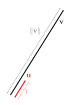
\includegraphics[width = 0.3\textwidth]{unit_vector}
}
\end{tabular}




\section*{Review of Cartesian coordinates}

\begin{tabular}{cc}
\parbox{0.5\textwidth}{
In the image to the right, the coordinates of the labeled points \(A\), \(B\), \(C\), \(D\), \(E\), \(F\), \(G\), \(H\), \(I\), \(J\), \(K\), \(L\), \(M\), \(N\), \(O\), \(P\), \(Q\), \(R\), \(S\), \(T\), \(U\), and \(V\) are:
\begin{tabular}{cccc}
\(A(2, 0)\) & \(B(2, 3)\) & \(C(0, 0)\) & \(D(0, 3)\) \\ 
\(E(-3, 3)\) & \(F(0, -1)\) & \(G(-3, -1)\) & \(H(-3, -3)\) \\ 
\(I(3, -1)\) & \(J(3, -3)\) & \(K(6, -3)\) & \(L(6, 6)\) \\
\(M(3, 4)\) & \(N(3, 6)\) & \(O(-4, 4)\) & \(P(-4, 6)\) \\
\(Q(-6, 6)\) & \(R(-4, -4)\) & \(S(-6, -4)\) & \(T(-6, -6)\) \\
\(U(6, -4)\) & \(V(6, -6)\)
\end{tabular}
} & \parbox{0.5\textwidth}{
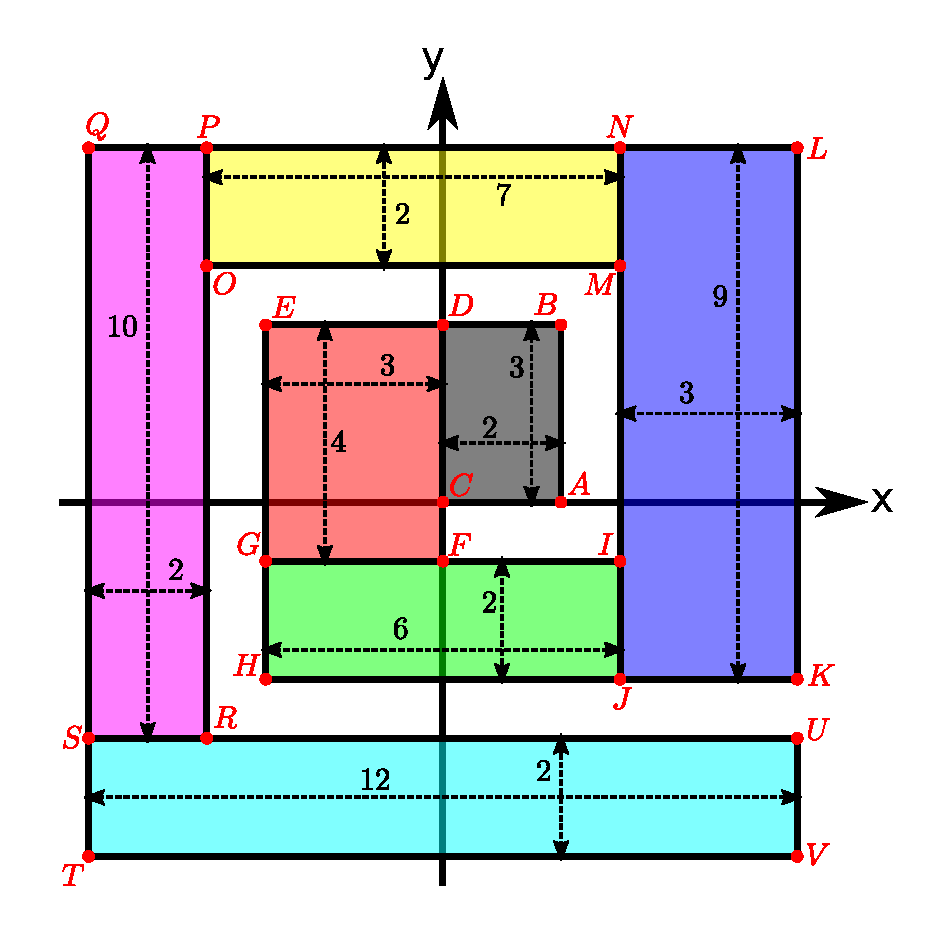
\includegraphics[width = 0.5\textwidth]{Cartesian_coordinates_example}
}
\end{tabular}

\begin{tabular}{cc}
\parbox{0.5\textwidth}{
Consider an arbitrary equation \(f(x,y) = g(x,y)\), where \(f(x,y)\) and \(g(x,y)\) are arbitrary expressions involving \(x\) and \(y\). The set of points that satisfy this equation forms a curve, where a point \((x,y)\) is included on the curve if and only if \((x,y)\) satisfies \(f(x,y) = g(x,y)\). This curve is referred to the {\bf graph} of \(f(x,y) = g(x,y)\) or the {\bf locus} of points that satisfies \(f(x,y) = g(x,y)\). \\
The purpose of the equation \(f(x,y) = g(x,y)\) is to distinguish between points that are part of the curve, and points that are not part of the curve. Given an arbitrary point \((x, y)\), the equation \(f(x,y) = g(x,y)\) is true if and only if point \((x, y)\) is part of the curve graphed by \(f(x,y) = g(x,y)\). \\
In the image on the right, the graph of the equation \(y = x^2\) is shown. In this case, \(f(x, y) = y\) and \(g(x, y) = x^2\). Given the point \((x, y) = (-1, 1)\) for example, \(y = 1\) and \(x^2 = 1\) so the equation is satisfied, and \((-1, 1)\) is part of the curve. Given the point \((x, y) = (2, 1)\) for example, \(y = 1\) and \(x^2 = 4\) so the equation is falsified, and \((2, 1)\) is not part of the curve. \\
This equation \(y = x^2\) is also equivalent to the equation \(x^2 - y = 0\), where \(f(x, y) = x^2 - y\) and \(g(x, y) = 0\).
} & \parbox{0.5\textwidth}{
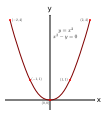
\includegraphics[width = 0.5\textwidth]{parabola}
}
\end{tabular}

\begin{tabular}{cc}
\parbox{0.5\textwidth}{
Consider a curve with the equation 
\[f(x,y) = g(x,y)\] 
Shifting this curve by a displacement of \(\langle a, b \rangle\), the equation of the new shifted curve can be derived as follows: If point \((x_\text{old}, y_\text{old})\) lies on the original curve, then point \((x_\text{new}, y_\text{new}) = (x_\text{old}+a, y_\text{old}+b)\) lies on the shifted curve. Point \((x_\text{old}, y_\text{old})\) satisfies the equation \(f(x_\text{old},y_\text{old}) = g(x_\text{old},y_\text{old})\). Since \((x_\text{old}, y_\text{old}) = (x_\text{new}-a, y_\text{new}-b)\), point \((x_\text{new}, y_\text{new})\) satisfies the equation \(f(x_\text{new} - a, y_\text{new} - b) = g(x_\text{new} - a, y_\text{new} - b)\). Therefore:
\[f(x-a, y-b) = g(x-a, y-b)\] 
is the equation of the graph of \(f(x,y) = g(x,y)\) shifted by the displacement \(\langle a, b \rangle\).
} & \parbox{0.5\textwidth}{
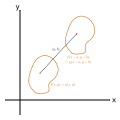
\includegraphics[width = 0.5\textwidth]{translation_of_curves}
}
\end{tabular}

\begin{tabular}{cc}
\parbox{0.5\textwidth}{
Consider a curve with the equation 
\[f(x,y) = g(x,y)\] 
Scaling the curve by a factor of \(k_x\) parallel to the \(x\)-axis, and by a factor of \(k_y\) parallel to the \(y\)-axis, the equation of the new scaled curve can be derived as follows: If point \((x_\text{old}, y_\text{old})\) lies on the original curve, then point \((x_\text{new}, y_\text{new}) = (k_x x_\text{old}, k_y y_\text{old})\) lies on the scaled curve. Point \((x_\text{old}, y_\text{old})\) satisfies the equation \(f(x_\text{old},y_\text{old}) = g(x_\text{old},y_\text{old})\). Since \((x_\text{old}, y_\text{old}) = (x_\text{new}/k_x, y_\text{new}/k_y)\), point \((x_\text{new}, y_\text{new})\) satisfies the equation \(f(x_\text{new}/k_x, y_\text{new}/k_y) = g(x_\text{new}/k_x, y_\text{new}/k_y)\). Therefore:
\[f(x/k_x, y/k_y) = g(x/k_x, y/k_y)\] 
is the equation of the graph of \(f(x,y) = g(x,y)\) scaled by a factor of \(k_x\) parallel to the \(x\)-axis, and scaled by a factor of \(k_y\) parallel to the \(y\)-axis.
} & \parbox{0.5\textwidth}{
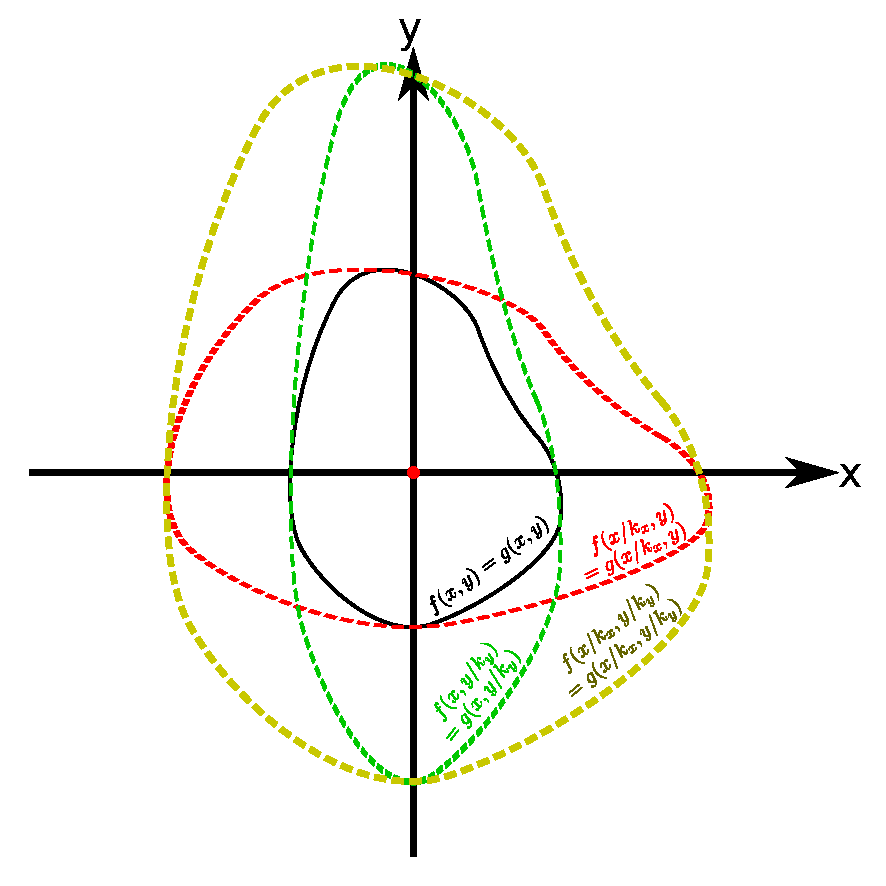
\includegraphics[width = 0.5\textwidth]{lateral_scaling_of_curves}
}
\end{tabular}




\section*{Lines}

Now will be described the equations whose graphs are {\bf lines}.

\begin{tabular}{cc}
\parbox{0.5\textwidth}{
Important to lines is the ``gradient" or ``slope" of the line. The slope quantifies the ``steepness" of the line, and is defined as the change in the \(y\)-coordinate for a change of \(1\) in the \(x\) coordinate. Given two points \(A(x_1, y_1)\) and \(B(x_2, y_2)\) and the line that passes through \(A\) and \(B\), the change of \(x_2 - x_1\) in the \(x\)-coordinate corresponds to a change of \(y_2 - y_1\) in the \(y\)-coordinate. The change in the \(y\)-coordinate per change of \(1\) in the \(x\)-coordinate is the gradient: 
\[m = \frac{y_2 - y_1}{x_2 - x_1}\] 
} & \parbox{0.5\textwidth}{
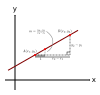
\includegraphics[width = 0.5\textwidth]{gradient}
}
\end{tabular}

\begin{tabular}{cc}
\parbox{0.5\textwidth}{
The equation of a line \(L_0\) with a gradient of \(m\) and that passes through the origin point is \(y = mx\). Starting at \((0,0)\), increasing the \(x\)-coordinate to \(x\) changes the \(y\)-coordinate to \(y = mx\). Now if it is known that line \(L\) passes through the point \((x_0, y_0)\), then displacing line \(L_0\) by a displacement of \(\langle x_0, y_0 \rangle\) so that the point at the origin has been moved to \((x_0, y_0)\), the new equation for line \(L\) is \(y - y_0 = m(x - x_0)\). This equation can also easily be observed by noting that if \((x_0, y_0)\) lies on \(L\), then increasing \(x_0\) by the amount \(x - x_0\) to \(x\), will also increase \(y_0\) by the amount \(y - y_0 = m(x - x_0)\) by definition of the gradient. Therefore:
\[y - y_0 = m(x - x_0)\] 
is the equation of line \(L\).
} & \parbox{0.5\textwidth}{
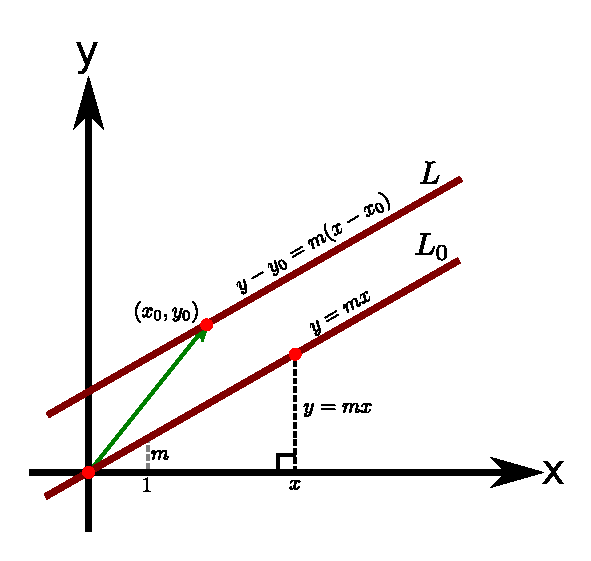
\includegraphics[width = 0.5\textwidth]{gradient_3}
}
\end{tabular}

\begin{tabular}{cc}
\parbox{0.5\textwidth}{
If the point that line \(L\) passes through is the \(y\)-intercept \((0, c)\), then the equation of line \(L\) is:
\[y - c = m(x - 0) \iff y = mx + c\]
The equation \(y = mx + c\) is the most common form of equation for a line. The equation \(y - y_0 = m(x - x_0)\) will often be manipulated to \(y = mx + (y_0 - mx_0)\).
} & \parbox{0.5\textwidth}{
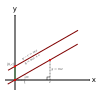
\includegraphics[width = 0.5\textwidth]{gradient_4}
}
\end{tabular}

The standard equation of the line that is being used is:
\[y = mx + c\]
where \(m\) is the gradient of the line, and \(c\) is the \(y\)-axis intercept. The slope \(m\) is the change in \(y\) \emph{per unit change} in \(x\): \(m = \frac{\Delta y}{\Delta x} = \frac{y_2 - y_1}{x_2 - x_1}\) where \((x_1, y_1)\) and \((x_2, y_2)\) are points from the line. The \(y\)-axis intercept \(c\) is the value attained by \(y\) when the line crosses the \(y\)-axis, which occurs when \(x = 0\). 

Given two points \(A(x_1, y_1)\) and \(B(x_2, y_2)\), the process of finding the equation of the line \(L\) that passes through points \(A\) and \(B\) can be summarized as follows: 
\begin{itemize}
\item Compute the slope \(m\) of line \(L\): 
\[m = \frac{y_2 - y_1}{x_2 - x_1}\]
\item Start with \(y = mx\), which is the equation of a line with a slope of \(m\) that contains the origin \((0, 0)\). Move this line through a displacement of \(\langle x_1, y_1 \rangle\) so that the origin is moved to point \(A\). This results in an equation for line \(L\):
\[y - y_1 = m(x - x_1)\]
Alternately, the line \(y = mx\) can be moved through the displacement \(\langle x_2, y_2 \rangle\) so that the origin is moved to point \(B\). This results in an {\bf equivalent} equation for line \(L\):
\[y - y_2 = m(x - x_2)\]
\item Solve the equation for \(y\) as an expression of \(x\). This equation will have the desired form 
\[y = mx + c\]
\end{itemize}

\textbf{Examples:}
\begin{itemize}
%%%%%%%%%%%%%%%%%%%%%%%%
\item Start with the two points \(A(-2, -5)\) and \(B(3, 8)\). The slope of the line that connects points \(A\) and \(B\) is \(m = \frac{8 - (-5)}{3 - (-2)} = \frac{13}{5}\). Using point \(A\), the equation of the line that contains both \(A\) and \(B\) is: 
\[y - (-5) = \frac{13}{5}(x - (-2)) \iff y = -5 + (\frac{13}{5}x + \frac{26}{5}) \iff y = \frac{13}{5}x + \frac{1}{5}\]
The equation of the line that contains both \(A\) and \(B\) is:
\[y = \frac{13}{5}x + \frac{1}{5}\]
To check that \(A\) and \(B\) are on this line, for point \(A(-2, -5)\) the equation becomes \(-5 = \frac{13}{5}(-2) + \frac{1}{5} \iff -5 = \frac{-25}{5} \iff -5 = -5\). For point \(B(3, 8)\) the equation becomes \(8 = \frac{13}{5}(3) + \frac{1}{5} \iff 8 = \frac{40}{5} \iff 8 = 8\).
%%%%%%%%%%%%%%%%%%%%%%%%
\item Start with the two points \(A(-3,4)\) and \(B(4,-2)\). The slope of the line that connects points \(A\) and \(B\) is \(m = \frac{(-2) - 4}{4 - (-3)} = \frac{-6}{7}\). Using point \(A\), the equation of the line that contains both \(A\) and \(B\) is: 
\[y - 4 = -\frac{6}{7}(x - (-3)) \iff y = 4 + (-\frac{6}{7}x - \frac{18}{7}) \iff y = -\frac{6}{7}x + \frac{10}{7}\]
The equation of the line that contains both \(A\) and \(B\) is:
\[y = -\frac{6}{7}x + \frac{10}{7}\]
To check that \(A\) and \(B\) are on this line, for point \(A(-3, 4)\) the equation becomes \(4 = -\frac{6}{7}(-3) + \frac{10}{7} \iff 4 = \frac{28}{7} \iff 4 = 4\). For point \(B(4, -2)\) the equation becomes \(-2 = -\frac{6}{7}(4) + \frac{10}{7} \iff -2 = -\frac{14}{7} \iff -2 = -2\).
%%%%%%%%%%%%%%%%%%%%%%%%
\item Start with the two points \(A(1,-4)\) and \(B(-5,2)\). The slope of the line that connects points \(A\) and \(B\) is \(m = \frac{2 - (-4)}{(-5) - 1} = \frac{6}{-6} = -1\). Using point \(A\), the equation of the line that contains both \(A\) and \(B\) is: 
\[y - (-4) = -1 \cdot (x - 1) \iff y = -4 + (-x + 1) \iff y = -x - 3\]
The equation of the line that contains both \(A\) and \(B\) is:
\[y = -x - 3\]
To check that \(A\) and \(B\) are on this line, for point \(A(1,-4)\) the equation becomes \(-4 = -1 - 3 \iff -4 = -4\). For point \(B(-5,2)\) the equation becomes \(2 = -(-5) - 3 \iff 2 = 2\).
%%%%%%%%%%%%%%%%%%%%%%%%
\item Start with the two points \(A(5,2)\) and \(B(-4,-1)\). The slope of the line that connects points \(A\) and \(B\) is \(m = \frac{(-1) - 2}{(-4) - 5} = \frac{-3}{-9} = \frac{1}{3}\). Using point \(A\), the equation of the line that contains both \(A\) and \(B\) is: 
\[y - 2 = \frac{1}{3}(x - 5) \iff y = 2 + (\frac{1}{3}x - \frac{5}{3}) \iff y = \frac{1}{3}x + \frac{1}{3}\]
The equation of the line that contains both \(A\) and \(B\) is:
\[y = \frac{1}{3}x + \frac{1}{3}\]
To check that \(A\) and \(B\) are on this line, for point \(A(5,2)\) the equation becomes \(2 = \frac{1}{3}(5) + \frac{1}{3} \iff 2 = \frac{6}{3} \iff 2 = 2\). For point \(B(-4,-1)\) the equation becomes \(-1 = \frac{1}{3}(-4) + \frac{1}{3} \iff -1 = \frac{-3}{3} \iff -1 = -1\).
\end{itemize}



\subsection*{Converting equations to $y = mx + c$}

Sometimes, the equation of a line will not be given in the form \(y = mx + c\). When this is the case, the equation must be manipulated until the form \(y = mx + c\) is attained. 

\textbf{Examples:}
\begin{itemize}
%%%%%%%%%%%%%
\item Given the equation \(3x - 7y = 14\), 
\[3x - 7y = 14 \iff 7y = 3x - 14 \iff y = \frac{3}{7}x - 2\]
so \(3x - 7y = 14\) is equivalent to \(y = \frac{3}{7}x - 2\)
%%%%%%%%%%%%%
\item Given the equation \(-10x + 5y = 15\),
\[-10x + 5y = 15 \iff 5y = 10x + 15 \iff y = 2x + 3\]
so \(-10x + 5y = 15\) is equivalent to \(y = 2x + 3\)
%%%%%%%%%%%%%
\item Given the equation \(6x - 7y + 13 = x + 3y - 7\), 
\[6x - 7y + 13 = x + 3y - 7 \iff 5x + 20 = 10y \iff y = \frac{1}{2}x + 2\] 
so \(6x - 7y + 13 = x + 3y - 7\) is equivalent to \(y = \frac{1}{2}x + 2\)
\end{itemize}




\subsection*{Vertical lines}

When a line is vertical, its slope is \(m = \infty\). The equation that quantifies a vertical line cannot take the form \(y = mx + c\), and instead has the form \(x = a\) where \(a\) is the value that \(x\) is fixed to. Examples include:
\begin{itemize}
\item \(x = -1\) is the equation of a vertical line where the \(x\)-coordinate is \(-1\) for all points on the line.
\item \(x = 3\) is the equation of a vertical line where the \(x\)-coordinate is \(3\) for all points on the line.
\item \(x = 1\) is the equation of a vertical line where the \(x\)-coordinate is \(1\) for all points on the line.
\end{itemize}



\subsection*{Perpendicular lines} 

\begin{tabular}{cc}
\parbox{0.5\textwidth}{
Consider two {\bf perpendicular} lines \(L_1\) and \(L_2\). Let the slopes of lines \(L_1\) and \(L_2\) be respectively denoted by \(m_1\) and \(m_2\). In the image on the right, there are two triangles. The upper triangle illustrates the slope of line \(L_1\), with a change in the \(x\)-coordinate of \(1\), and a change in the \(y\)-coordinate of \(m_1 \cdot 1 = m_1\). The lower triangle is congruent to the upper triangle, albeit rotated by \(90^\circ\). The lower triangle illustrates the slope of \(L_2\), with a change in the \(x\)-coordinate of \(m_1\), and a change in the \(y\)-coordinate of \(-1\). The slope of \(L_2\) is \(m_2 = \frac{-1}{m_1}\). Therefore:
\[m_2 = -\frac{1}{m_1}\]
} & \parbox{0.5\textwidth}{
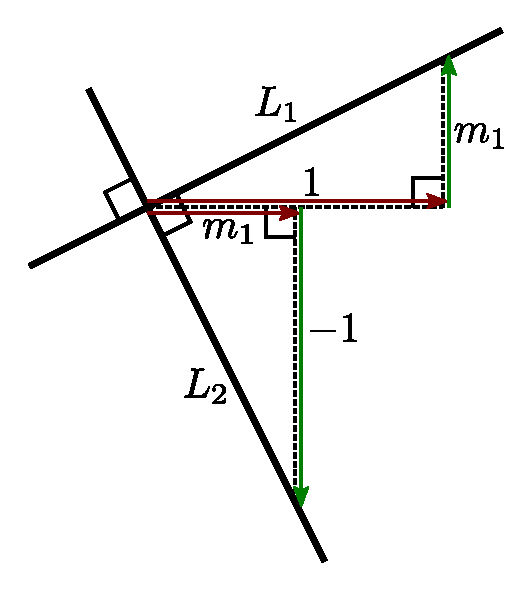
\includegraphics[width = 0.5\textwidth]{perpendicular_slope}
}
\end{tabular}

\textbf{Examples:}
\begin{itemize}
%%%%%%%%%%%%%
\item Consider the points \(A(-3, -1)\); \(B(5, 3)\); and \(C(4, -4)\). What is sought is the equation of a line \(L_2\) that passes through point \(C\) and is {\bf perpendicular} to the line \(L_1\) that passes through points \(A\) and \(B\). \\
The slope \(m_1\) of line \(L_1\) is \(m_1 = \frac{3 - (-1)}{5 - (-3)} = \frac{4}{8} = \frac{1}{2}\). The slope \(m_2\) of line \(L_2\) is \(m_2 = -\frac{1}{m_1} = -2\). The line \(y = -2x\) passes through the origin, and moving the origin to point \(C\) yields the following equation for \(L_2\):
\[y - (-4) = -2(x - 4) \iff y = -4 + (-2x + 8) = -2x + 4\]
The equation for \(L_2\) is: 
\[y = -2x + 4\]
%%%%%%%%%%%%%
\item Consider the points \(A(3, -2)\); \(B(-2, 4)\); and \(C(8, -9)\). What is sought is the equation of a line \(L_2\) that passes through point \(C\) and is {\bf perpendicular} to the line \(L_1\) that passes through points \(A\) and \(B\). \\
The slope \(m_1\) of line \(L_1\) is \(m_1 = \frac{4 - (-2)}{-2 - 3} = \frac{6}{-5} = -\frac{6}{5}\). The slope \(m_2\) of line \(L_2\) is \(m_2 = -\frac{1}{m_1} = \frac{5}{6}\). The line \(y = \frac{5}{6}x\) passes through the origin, and moving the origin to point \(C\) yields the following equation for \(L_2\):
\[y - (-9) = \frac{5}{6}(x - 8) \iff y = -9 + (\frac{5}{6}x - \frac{20}{3}) = \frac{5}{6}x - \frac{47}{3}\]
The equation for \(L_2\) is: 
\[y = \frac{5}{6}x - \frac{47}{3}\]
\end{itemize}



\subsection*{Plotting lines: finding the intercept points}

It is often useful to draw a line from its equation to get a better understanding of its shape and behavior. One of the most efficient approaches to plotting a line to is to first compute the \(x\) and \(y\) intercepts, and then plot the intercept points and draw a line that passes through the two intercept points. Given a line whose equation is \(y = mx + c\), the \(y\) intercept point is clearly \((0, c)\). To find the \(x\) intercept point, the value of \(x\) that causes \(y = 0\) must be found:
\[0 = mx + c \iff x = -\frac{c}{m}\]  
this yields the intercept point \((-c/m, 0)\).

\textbf{Examples:}
\begin{itemize}
%%%%%%%%%%%%%
\item The line \(y = \frac{2}{3}x + 5\) intersects the \(y\) axis at the point \((0, 5)\), and intersects the \(x\) axis when \(y = 0\). \(\frac{2}{3}x + 5 = 0 \iff x = -\frac{15}{2}\) so the \(x\) intercept is \((-15/2, 0)\). Draw a line through the points \((0, 5)\) and \((-15/2, 0)\) to plot the line \(y = \frac{2}{3}x + 5\).
%%%%%%%%%%%%%
\item The line \(y = -\frac{1}{2}x + 7\) intersects the \(y\) axis at the point \((0, 7)\), and intersects the \(x\) axis when \(y = 0\). \(-\frac{1}{2}x + 7 = 0 \iff x = 14\) so the \(x\) intercept is \((14, 0)\). Draw a line through the points \((0, 7)\) and \((14, 0)\) to plot the line \(y = -\frac{1}{2}x + 7\).
%%%%%%%%%%%%%
\item The line \(y = -\frac{3}{8}x + 6\) intersects the \(y\) axis at the point \((0, 6)\), and intersects the \(x\) axis when \(y = 0\). \(-\frac{3}{8}x + 6 = 0 \iff x = 16\) so the \(x\) intercept is \((16, 0)\). Draw a line through the points \((0, 6)\) and \((16, 0)\) to plot the line \(y = -\frac{3}{8}x + 6\).
\end{itemize}





\section*{Circles}

\subsection*{Distance between two points}

\begin{tabular}{cc}
\parbox{0.5\textwidth}{
Given two points \(A(x_1, y_1)\) and \(B(x_2, y_2)\), the displacement from \(A\) to \(B\) is \(\mathbf{d} = \langle x_2 - x_1, y_2 - y_1 \rangle\). The distance from \(A\) to \(B\) is the length of this displacement which is \(d = \|\mathbf{d}\| = \sqrt{(x_2 - x_1)^2 + (y_2 - y_1)^2}\). \\
\textbf{Examples:}
\begin{itemize}
\item The distance from \(A(-3,2)\) to \(B(4,-1)\) is \(d = \sqrt{7^2 + (-3)^2} = \sqrt{49 + 9} = \sqrt{58} \approx 7.61577\)
\item The distance from \(A(11,-2)\) to \(B(3,5)\) is \(d = \sqrt{(-8)^2 + 7^2} = \sqrt{64 + 49} = \sqrt{113} \approx 10.6301\)
\item The distance from \(A(5,8)\) to \(B(7,0)\) is \(d = \sqrt{2^2 + (-8)^2} = \sqrt{4 + 64} = \sqrt{68} = 2\sqrt{17} \approx 8.24621\)
\end{itemize}
}
& \parbox{0.5\textwidth}{
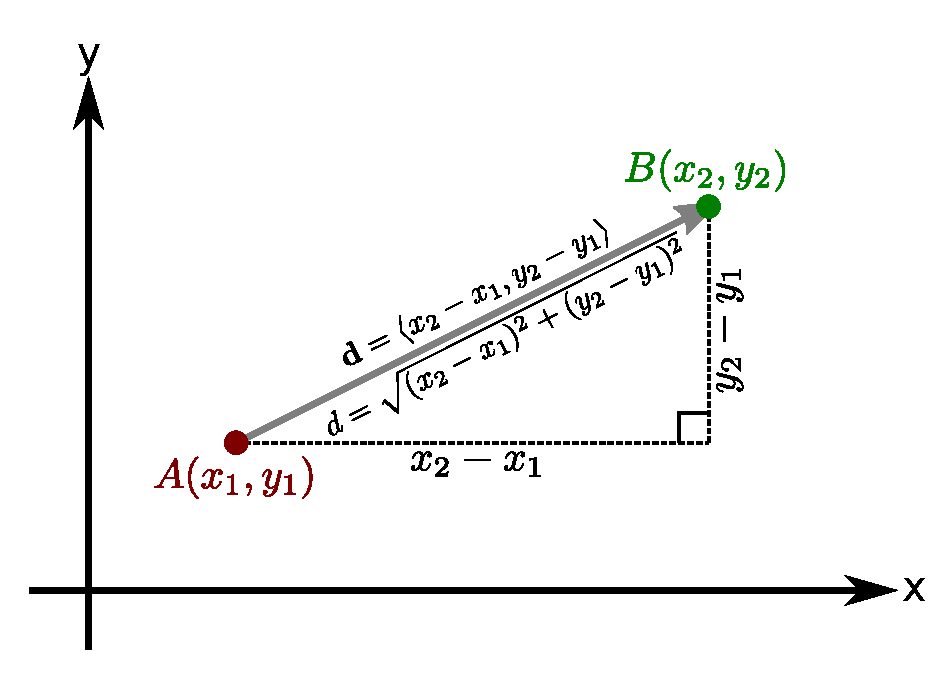
\includegraphics[width = 0.5\textwidth]{distance_between_points}
}
\end{tabular}


\subsection*{Midpoint between two points}

\begin{tabular}{cc}
\parbox{0.5\textwidth}{
Given two points \(A(x_1, y_1)\) and \(B(x_2, y_2)\), the ``midpoint" \(C\) that is exactly halfway between points \(A\) and \(B\) is computed as follows: The displacement from point \(A\) to point \(B\) is \(\mathbf{d} = \langle x_2 - x_1, y_2 - y_1 \rangle\). The ``midpoint" \(C\) is reached from \(A\) by a displacement of \(\frac{\mathbf{d}}{2} = \langle \frac{x_2 - x_1}{2}, \frac{y_2 - y_1}{2} \rangle\). Shifting \(A\) by the displacement of \(\frac{\mathbf{d}}{2}\) gives \(C(x_1 + \frac{x_2 - x_1}{2}, y_1 + \frac{y_2 - y_1}{2}) = C(\frac{x_1 + x_2}{2}, \frac{y_1 + y_2}{2})\). Therefore the midpoint is:
\[C(\frac{x_1 + x_2}{2}, \frac{y_1 + y_2}{2})\]
\textbf{Examples:}
\begin{itemize}
\item The midpoint between \(A(-3,2)\) and \(B(4,-1)\) is \(C(\frac{1}{2},\frac{1}{2})\)
\item The midpoint between \(A(11,-2)\) and \(B(3,5)\) is \(C(7,\frac{3}{2})\)
\item The midpoint between \(A(5,8)\) and \(B(7,0)\) is \(C(6,4)\)
\end{itemize}
}
& \parbox{0.5\textwidth}{
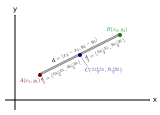
\includegraphics[width = 0.5\textwidth]{midpoint_formula}
}
\end{tabular}


\subsection*{The equations of circles}

\begin{tabular}{cc}
\parbox{0.5\textwidth}{
Given a radius \(R > 0\), a circle of radius \(R\) that is centered on the origin is the set (locus) of all points that are a distance of \(R\) from the origin. A point \((x,y)\) is a distance of \(R\) from the origin if and only if \(\sqrt{x^2 + y^2} = R\) which is equivalent to \(x^2 + y^2 = R^2\). The equation 
\[x^2 + y^2 = R^2\] 
defines a circle of radius \(R\) that is centered on the origin. \\ 
Centering a circle of radius \(R\) on the point \((a,b)\) requires that the origin centered circle be shifted a displacement of \(\langle a, b \rangle\). This yields the equation
\[(x-a)^2 + (y-b)^2 = R^2\] 
which defines a circle of radius \(R\) that is centered on the point \((a,b)\).
} & \parbox{0.5\textwidth}{
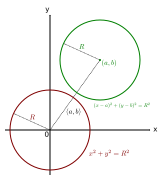
\includegraphics[width = 0.5\textwidth]{circle}
}
\end{tabular}


\textbf{Examples:}
\begin{itemize}
%%%%%%
\item Given a point \(A(1,2)\) and radius of \(R = 3\), a circle of radius \(R\) centered on point \(A\) has the equation:
\[(x-1)^2 + (y-2)^2 = 9\] 
%%%%%%
\item Given a point \(A(-3,3)\) and radius of \(R = 4\), a circle of radius \(R\) centered on point \(A\) has the equation:
\[(x+3)^2 + (y-3)^2 = 16\] 
%%%%%%
\item Given points \(A(2,6)\) and \(B(-1,-1)\), a circle that is centered of point \(A\) and that \emph{passes through} point \(B\) is sought. The radius \(R\) of this circle is the distance between points \(A\) and \(B\). \(R = \sqrt{(-3)^2 + (-7)^2} = \sqrt{9 + 49} = \sqrt{58}\). The circle's equation is: 
\[(x - 2)^2 + (y - 6)^2 = 58\]
%%%%%%
\item Given points \(A(-4,1)\) and \(B(6,9)\), a circle whose diameter is the line segment from \(A\) to \(B\) is sought. The radius \(R\) of the circle is half the distance between points \(A\) and \(B\). \(R = \frac{1}{2}\sqrt{10^2 + 8^2} = \frac{1}{2}\sqrt{100 + 64} = \frac{1}{2}\sqrt{164} = \sqrt{41}\). The circle is centered on the midpoint \(C\) between points \(A\) and \(B\): \(C(1,5)\). The circle's equation is:
\[(x - 1)^2 + (y - 5)^2 = 41\]
%%%%%%
\item Given points \(A(3,8)\) and \(B(-7,10)\), a circle whose diameter is the line segment from \(A\) to \(B\) is sought. The radius \(R\) of the circle is half the distance between points \(A\) and \(B\). \(R = \frac{1}{2}\sqrt{(-10)^2 + 2^2} = \frac{1}{2}\sqrt{100 + 4} = \frac{1}{2}\sqrt{104} = \sqrt{26}\). The circle is centered on the midpoint \(C\) between points \(A\) and \(B\): \(C(-2,9)\). The circle's equation is:
\[(x + 2)^2 + (y - 9)^2 = 26\]
\end{itemize}





\end{document}











